%!TEX root = ../main.tex
\chapter{Methodology}
\label{chap:methodology}
\section{Overview}
User requirement changes continuously and relying on a methodology helped organize the development into phases, providing a more flexible development. This chapter will detail the approach that will be used in the project, with the aim of outlining how each one will lead to achieving the objectives.
\section{Agile}
\say{Agile methodologies are purported to imbue flexibility in
software development projects, thereby enabling software
development teams to perform more effectively}, \cite{maruping2009control}.
 They share the property of iterative incremental development that tackles requirement changes quickly, satisfy customer and produce quality products, \cite{6633925}.
Many Agile methodologies has been introduced, of these, XP and scrum are the most popular.

	\begin{figure}[h]
	\centering
	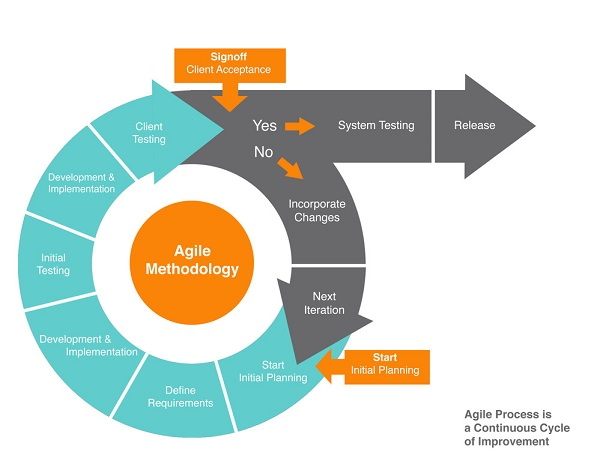
\includegraphics[width=0.4\textheight]{Agile}
	\caption{Agile Lifecycle}
	\label{fig:agile_lifecycle}
\end{figure}

\subsection{XP}
Extreme Programming is a software development methodology designed to improve the quality of software and its ability to properly adapt to the changing needs of the consumer, \cite{ExtremeP63:online}.
Similar to other Agile Methods of development, XP aims to provide iterative and frequent small releases throughout the project, allowing both team members and customers to examine and review the project’s progress throughout the entire System Development Life Cycle(SDLC).

Extreme Programming amends a software project in five essential ways; communication, simplicity, feedback, respect, and courage. Extreme Programmers get feedback by testing their software from day one and distribute the system to the customers as early as possible, implementing changes as suggested by the customer.
\subsection{Scrum}
Scrum is a subset of Agile and one of the most popular process frameworks for implementing Agile. It is an iterative software development model used to manage complex software and product development. Fixed-length iterations, called sprints lasting one to two weeks long, allow the team to ship software on a regular cadence. At the end of each sprint, stakeholders and team members meet to plan next steps, \cite{FullComp27:online}.
 
Scrum follows a set of rules; a scrum master has to be appointed, he/she normally conducts scrum meetings and makes decision. 
Scrum also relies heavily on backlog(list of features, bug fixes and improvement). These meetings aims to get developers to be more productive with an appropriate amount of supervision to handle issues that may arise.

\section{Cowboy}
 Most methodologies focusses on groups of people to collaborate efficaciously to indite a software project, what about solo programmers? Cowboy was designed to fill this void. 

Cowboy is an agile system that benefits from agile methodologies,
customer centered approach and helps the programmer to stay focused while meeting customer needs. It is an iterative approach, meaning it adds features and fixes bugs of previous cycle.

Finally, cowboy suggest that the artefact should be kept simple and adequate, encapsulate the core ideas, which are subject to change(or even elimination) as requirement change, so not much time should be lost perfecting them, \cite{hollar2006cowboy}.

According to Hollar, developers who had relied on this methodology includes; Alan Turing, viewed as the precursor to the modern programmer, Bill Gates, essentially when inditing MS Basic.

\section{How Agile Helped Cowboy}
Cowboy relies on having a customer(or at least someone knowledgeable to represent the client interest). In this thesis it will be the supervisor of the project and a potential client interested in the development of the artefact. Their feedback should weigh somehow in deciding the order in which to add the features. The developer has autonomy over the development process and the authority to refuse a feature suggested by the client, which if pursued may take away vital time.

During development, cowboy suggests developers should target the huge problem first then move on to minor issues, code refactoring should be done during each cycle.

The combination with the agile methodology mentioned above, helped in the successful development of the application.

Deniz Centinkaya, agreed to act as the supervisor of this project and it was planned to hold weekly meetings, and continuous communication through email was relied on as well. 

\section{Project Plan}
In order to have a successful project, a Gantchart has been developed. The chart breaks down the project into sub projects and provides the start and the end date of that particular sub project, refer to appendix \ref{gantchart}.
